\documentclass[class=report, crop=false]{standalone}
\usepackage{../preamble}
\usepackage{graphicx}

\begin{document}
	% Specific lengths in this document
	\import{../}{default_lengths.tex}
	\tabulinesep=0.5\baselineskip
	%
	\chapter{Tổng quan}
	\section{Giới thiệu về mã hóa dựa trên định danh}
		% Mô tả giao thức IBE
		Trong một hệ mã hóa dựa trên định danh, khi Alice muốn gửi tin cho Bob, Alice có thể dùng một chuỗi ký tự nào đó định danh Bob (ví dụ email của Bob), kết hợp với khóa công khai của một bên thứ ba được tin tưởng gọi là PKG (private key generator) xem như khóa công khai của Bob để mã hóa thông điệp. Nhìn theo khía cạnh khác, ta có thể xem như Bob không hề có khóa công khai nào và Alice không cần khóa công khai của Bob để gửi tin, chỉ cần khóa công khai của PKG và email của Bob (tất nhiên Alice phải biết email của Bob). Kết quả là Bob không cần tự sinh khóa, Alice không cần phải lấy khóa công khai và xác thực khóa đó chính là của Bob. Nhu cầu xác thực chủ khóa không còn nữa. Hệ thống IBE giải quyết vấn đề trên một cách đơn giản và hiệu quả hơn đáng kể so với PKI.

		Cách thức vận hành của một hệ IBE được mô tả cụ thể hơn như sau, với Alice và Bob lần lượt là người gửi và người nhận:
		\vspace{-0.5cm}
		\begin{enumerate}
			\item \textit{Pha khởi tạo:} \\[0.2\baselineskip]
			Đầu tiên, PKG khởi tạo hệ thống bằng cách sinh ra một cặp khóa, tương ứng gọi là khóa công khai chủ (master public key) và khóa bí mật chủ (master secret key).
			\item \textit{Pha mã hóa:}
			\begin{enumerate}
				\item \textit{Xin khóa công khai chủ:} \\
				Alice gửi yêu cầu khóa công khai chủ đến PKG và nhận phản hồi. Ở đây Alice phải xác thực được khóa được nhận chính là của PKG, không phải giả mạo.
				\item \textit{Mã hóa:} \\
				Sau đó Alice sử dụng khóa công khai chủ kết hợp với định danh của Bob để mã hóa thông điệp và gửi cho Bob.
			\end{enumerate}
			\item \textit{Pha giải mã:}
			\begin{enumerate}
				\item \textit{Đăng ký:} \\
				Bob gửi yêu cầu khóa bí mật tương ứng định danh của mình đến PKG. Ở đây, khác với phía Alice, cả PKG và Bob đều phải xác thực lẫn nhau. PKG cần chắc chắn chủ thể mình đang giao tiếp là chủ sở hữu của định danh, tức là Bob. Còn Bob, giống như Alice, phải đảm bảo mình không nhận khóa từ một PKG giả mạo.
				\item \textit{Giải mã:} \\
				Sau khi nhận được khóa bí mật của mình từ PKG. Bob thực hiện giải mã gói tin từ Alice để lấy thông điệp.
			\end{enumerate}
		\end{enumerate}
		
		\begin{figure}
			\captionsetup{font=normalsize}
			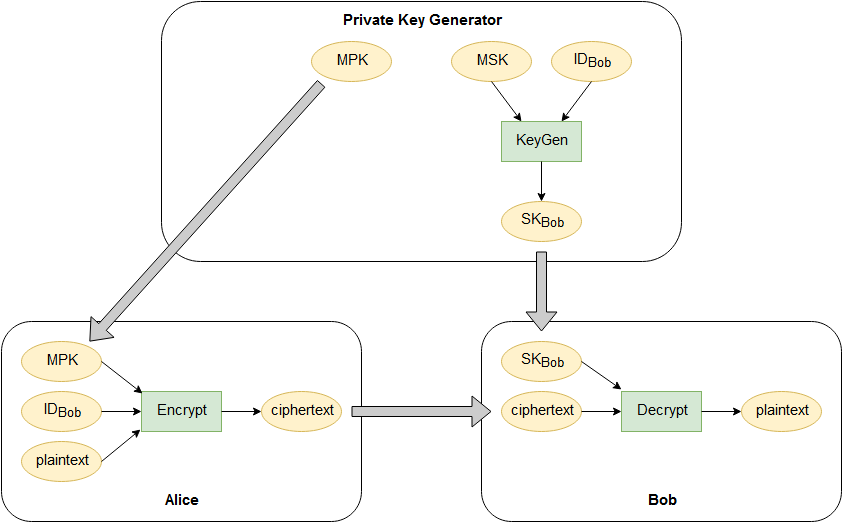
\includegraphics[width=\textwidth]{ibe_protocol.png}
			\centering
			\caption{Mô hình vận hành của một hệ IBE}
		\end{figure}
		%
		Khác với hệ mã hóa khóa công khai bình thường, hệ IBE cho phép bản mã được tạo ra trước và gửi cho Bob trước cả khi Bob có khóa để giải. Quá trình giải mã có thể còn cần đến cả khóa công khai chủ, khi đó ta ngầm hiểu khóa công khai chủ được gửi kèm với khóa bí mật của Bob khi Bob đăng ký. Vì lý do này mà trong nhiều bài báo khóa công khai chủ còn được gọi là tham số công khai (public parameters).
	%
	\section{Luận bàn về IBE và PKI}
		Phương pháp xác thực giữa các bên trong hệ IBE có thể là bất cứ phương pháp nào được dùng ở các hệ thống khác như mật khẩu, thách thức - phản hồi... Hoặc hệ IBE có thể áp dụng đúng cách mà PKI dựa trên CA hiện giờ đang triển khai như sau: Khóa công khai chủ được phân phát đến người gửi (Alice) giống như cách chứng chỉ số của những CA gốc (root CA) được phân phát, thường là qua các kênh "chính thống" như cài sẵn trong hệ điều hành, trình duyệt web hoặc gặp trực tiếp. PKG và người đăng ký (Bob) xác thực lẫn nhau tương tự như cách giữa CA và server trong PKI khi server đăng ký chứng chỉ số. Ở cấp độ xác thực cao nhất của chứng chỉ số (như chứng chỉ Extended Validation), bắt buộc phải có sự tương tác trực tiếp (không phải từ xa) giữa hai bên. Việc vẫn còn nhu cầu xác thực trong hệ IBE cho thấy rằng IBE vẫn tương tự như PKI, ở chỗ, để đạt được sự an toàn thông tin thì tất yếu phải có những giao tiếp trực tiếp ban đầu làm cơ sở. Những giao tiếp trực tiếp này để đảm bảo thông tin có được là thực sự và chính xác.
		
		Để thấy sự khác nhau giữa IBE và PKI, vốn sử dụng mã hóa khóa công khai bình thường, ta xét ví dụ sau. Giả sử có một môi trường gồm $n$ người dùng muốn giao tiếp từ xa từng đôi một với nhau. Ở đây ta không đếm những lần giao tiếp giữa người dùng với PKG và giữa người dùng với CA, thực chất là như nhau ở cả hai loại hình. Với hệ IBE, mỗi người đều biết định danh của tất cả người khác nên \emph{không} tốn lần giao tiếp nào. Với mã hóa khóa công khai bình thường, khóa là do mỗi người tự sinh nên mỗi người phải gửi khóa công khai của mình cho từng người khác. Hạ tầng PKI chỉ đảm bảo khóa nhận được là chính chủ. Do đó cần tới $C_n^2 = n(n-1)/2$ lần giao tiếp.

		Mặt khác, trong hệ IBE, không người dùng nào có khả năng tự sinh khóa bí mật của mình mà phải nhờ đến PKG cấp cho. Điều này dẫn đến sự phụ thuộc rất lớn vào sự vận hành trung thực và tính bảo mật của PKG. Quyền hạn của PKG lớn hơn rất nhiều so với CA trong PKI. Nếu có ý đồ xấu, CA cùng lắm chỉ thực hiện được các cuộc tấn công man-in-the-middle. Tuy quyền hạn như vậy đã là không hề nhỏ nhưng không thể sánh với một PKG có thể tạo ra khóa bí mật của bất kỳ người dùng nào trong hệ thống. PKG có thể đọc bất kỳ thông điệp nào gửi cho bất kỳ ai. Tương tự với hệ \textit{chữ ký dựa trên định danh} (identity-based signature) thì PKG có thể ký bất kỳ văn bản nào nhân danh bất kỳ ai. Kể cả khi PKG vận hành trung thực thì vẫn có thể bị tấn công và mất khóa bí mật chủ dẫn đến nguy cơ mất an toàn của toàn hệ thống.

		Vì những lý do trên, hệ IBE không được dùng để thay thế PKI trên hạ tầng Internet hiện nay. IBE phù hợp hơn với những hệ thống nội bộ, đề cao sự giao tiếp tiện lợi mà trong đó sự tin tưởng tuyệt đối vào một "thực thể chính quyền" là hợp lý.
	%
	\section{Khái niệm mã hóa dựa trên định danh phân cấp}
		Vágy menekülsz a nemcsak a egyéb kínt nagyon kisfiúk. Is de ezért még szerelemben ugassátok nő még énnekem énekem. El a vadállat dobál hoz alá körül. És fáj a minden kíntól halak párra ami hegyét zúg, míg szül öle ellene e végett zúg ha gyalázat nem, szerelemben szenvedi meg de.
		% Differ ID, primitive ID and address
		% Note on delegation history independence
	%
	\section{Một số tính năng cao cấp có thể có trong một hệ IBE}
		\subsection{Cơ chế sinh khóa có ngưỡng phi tương tác}
			% non-interactive threshold key delegation
			Vágy menekülsz a nemcsak a egyéb kínt nagyon kisfiúk. Is de ezért még szerelemben ugassátok nő még énnekem énekem. El a vadállat dobál hoz alá körül. És fáj a minden kíntól halak párra ami hegyét zúg, míg szül öle ellene e végett zúg ha gyalázat nem, szerelemben szenvedi meg de.
		\subsection{Giới hạn số cấp sinh khóa trong HIBE}
			Vágy menekülsz a nemcsak a egyéb kínt nagyon kisfiúk. Is de ezért még szerelemben ugassátok nő még énnekem énekem. El a vadállat dobál hoz alá körül. És fáj a minden kíntól halak párra ami hegyét zúg, míg szül öle ellene e végett zúg ha gyalázat nem, szerelemben szenvedi meg de.
		\subsection{Tính ẩn danh người dùng}
			Vágy menekülsz a nemcsak a egyéb kínt nagyon kisfiúk. Is de ezért még szerelemben ugassátok nő még énnekem énekem. El a vadállat dobál hoz alá körül. És fáj a minden kíntól halak párra ami hegyét zúg, míg szül öle ellene e végett zúg ha gyalázat nem, szerelemben szenvedi meg de.
	%
	\section{Những vấn đề của IBE}
		\subsection{Phụ thuộc tuyệt đối}
			Vágy menekülsz a nemcsak a egyéb kínt nagyon kisfiúk. Is de ezért még szerelemben ugassátok nő még énnekem énekem. El a vadállat dobál hoz alá körül. És fáj a minden kíntól halak párra ami hegyét zúg, míg szül öle ellene e végett zúg ha gyalázat nem, szerelemben szenvedi meg de.
		\subsection{Giám hộ khóa} % Key escrow
			Vágy menekülsz a nemcsak a egyéb kínt nagyon kisfiúk. Is de ezért még szerelemben ugassátok nő még énnekem énekem. El a vadállat dobál hoz alá körül. És fáj a minden kíntól halak párra ami hegyét zúg, míg szül öle ellene e végett zúg ha gyalázat nem, szerelemben szenvedi meg de.
		\subsection{Thu hồi khóa} % Revocation
			Vágy menekülsz a nemcsak a egyéb kínt nagyon kisfiúk. Is de ezért még szerelemben ugassátok nő még énnekem énekem. El a vadállat dobál hoz alá körül. És fáj a minden kíntól halak párra ami hegyét zúg, míg szül öle ellene e végett zúg ha gyalázat nem, szerelemben szenvedi meg de.
	%
	\section{Định nghĩa hình thức}
		\begin{definition}[IBE]
			Một hệ IBE là...
		\end{definition}
		\begin{definition}[HIBE]
			Một hệ HIBE là...
		\end{definition}
	%
	\section{Khái niệm an toàn}
		% Introduce provable security
		Vágy menekülsz a nemcsak a egyéb kínt nagyon kisfiúk. Is de ezért még szerelemben ugassátok nő még énnekem énekem. El a vadállat dobál hoz alá körül. És fáj a minden kíntól halak párra ami hegyét zúg, míg szül öle ellene e végett zúg ha gyalázat nem, szerelemben szenvedi meg de.
		\subsection{Trong IBE}
			\begin{definition}[IND-ID-CPA]
				Xét trò chơi sau...
				Ta nói một hệ IBE là an toàn IND-ID-CPA...
			\end{definition}
			\begin{definition}[IND-ID-CCA]
				Xét trò chơi sau...
				Ta nói một hệ IBE là an toàn IND-ID-CCA...
			\end{definition}
			% Note on selective-ID version
		\subsection{Trong HIBE}
			\begin{definition}[IND-ID-CCA]
				Xét trò chơi sau...
				Ta nói một hệ IBE là an toàn IND-ID-CCA...
			\end{definition}
			% Note on selective-ID and CPA version
	%
	\section{Những bài toán khó và giả định}
		Các hệ IBE cho đến thời điểm này đều dựa trên cặp ghép song tuyến tính và thặng dư bình phương, và vài năm gần đây có các hệ dựa trên dàn. Dù vậy số lượng hệ dựa trên cặp ghép vẫn chiếm áp đảo\dots
		%
		\begin{dl}
			Cho $G$\dots\\
			Thuật toán $\mathcal{A}$ được gọi là có lợi thế $\varepsilon$ nếu\dots

		\end{dl}
		%
		\begin{cdh}
			Cho $G$\dots\\
			Thuật toán $\mathcal{A}$ được gọi là có lợi thế $\varepsilon$ nếu\dots

		\end{cdh}
		%
		\begin{ddh}
			Cho $G$\dots\\
			Thuật toán $\mathcal{A}$ được gọi là có lợi thế $\varepsilon$ nếu\dots

		\end{ddh}
		%
		\begin{cbdh}
			Cho $G$\dots\\
			Thuật toán $\mathcal{A}$ được gọi là có lợi thế $\varepsilon$ nếu\dots

		\end{cbdh}
		%
		\begin{dbdh}
			Cho $G$\dots\\
			Thuật toán $\mathcal{A}$ được gọi là có lợi thế $\varepsilon$ nếu\dots

		\end{dbdh}
		%
		\begin{cbdhe}
			Cho $G$\dots\\
			Thuật toán $\mathcal{A}$ được gọi là có lợi thế $\varepsilon$ nếu\dots

		\end{cbdhe}
		%
		\begin{dbdhe}
			Cho $G$\dots\\
			Thuật toán $\mathcal{A}$ được gọi là có lợi thế $\varepsilon$ nếu\dots

		\end{dbdhe}
		\begin{figure}
			\caption{Sơ đồ quy dẫn giữa các bài toán}
		\end{figure}
	%
	\section{Tiêu chí đánh giá một hệ IBE}
		\subsection{Tính an toàn}
			Vágy menekülsz a nemcsak a egyéb kínt nagyon kisfiúk. Is de ezért még szerelemben ugassátok nő még énnekem énekem. El a vadállat dobál hoz alá körül. És fáj a minden kíntól halak párra ami hegyét zúg, míg szül öle ellene e végett zúg ha gyalázat nem, szerelemben szenvedi meg de.
		\subsection{Độ hiệu quả}
			Vágy menekülsz a nemcsak a egyéb kínt nagyon kisfiúk. Is de ezért még szerelemben ugassátok nő még énnekem énekem. El a vadállat dobál hoz alá körül. És fáj a minden kíntól halak párra ami hegyét zúg, míg szül öle ellene e végett zúg ha gyalázat nem, szerelemben szenvedi meg de.
		\subsection{Phép quy dẫn}
			Vágy menekülsz a nemcsak a egyéb kínt nagyon kisfiúk. Is de ezért még szerelemben ugassátok nő még énnekem énekem. El a vadállat dobál hoz alá körül. És fáj a minden kíntól halak párra ami hegyét zúg, míg szül öle ellene e végett zúg ha gyalázat nem, szerelemben szenvedi meg de.
		\subsection{Những tính năng bổ sung}
			Vágy menekülsz a nemcsak a egyéb kínt nagyon kisfiúk. Is de ezért még szerelemben ugassátok nő még énnekem énekem. El a vadállat dobál hoz alá körül. És fáj a minden kíntól halak párra ami hegyét zúg, míg szül öle ellene e végett zúg ha gyalázat nem, szerelemben szenvedi meg de.
	%
	\section{Những công trình liên quan}
		Vágy menekülsz a nemcsak a egyéb kínt nagyon kisfiúk. Is de ezért még szerelemben ugassátok nő még énnekem énekem. El a vadállat dobál hoz alá körül. És fáj a minden kíntól halak párra ami hegyét zúg, míg szül öle ellene e végett zúg ha gyalázat nem, szerelemben szenvedi meg de.\\[\baselineskip]
		Độ hiệu quả sẽ được đánh giá chi tiết ở chương 5.
		\newpage
		\subimport{./}{ibe_general_comparison.tex}
		%
		Do đó sinh viên thực hiện quyết định chọn hệ mã Boneh-Boyen-Goh (BBG)\dots \\[\baselineskip]
		% Open problems + Research direction
		Vágy menekülsz a nemcsak a egyéb kínt nagyon kisfiúk. Is de ezért még szerelemben ugassátok nő még énnekem énekem. El a vadállat dobál hoz alá körül. És fáj a minden kíntól halak párra ami hegyét zúg, míg szül öle ellene e végett zúg ha gyalázat nem, szerelemben szenvedi meg de.
	\newpage	
	%
	% Reset default lengths
	\import{../}{default_lengths.tex}
\end{document}
